\chapter{TETIS - Modelagem e Controle}


\section{Modelo}
O manipulador Tetis consiste basicamente de um braço planar de três elos com uma rotação adicional ao redor do eixo do plano. Também pode ser visto como um braço antropomórfico com uma junta de revolução adicional ao final da cadeia, com o eixo paralelo às duas anteriores. O projeto mecânico faz com que a extremidade do efetuador final não esteja exatamente alinhada com as juntas, o que é levado em conta no último elo. O esquema na figura \ref{fig:modelo_tetis} ilustra o modelo de elos e juntas. 
\begin{figure}[!ht]
\centering
  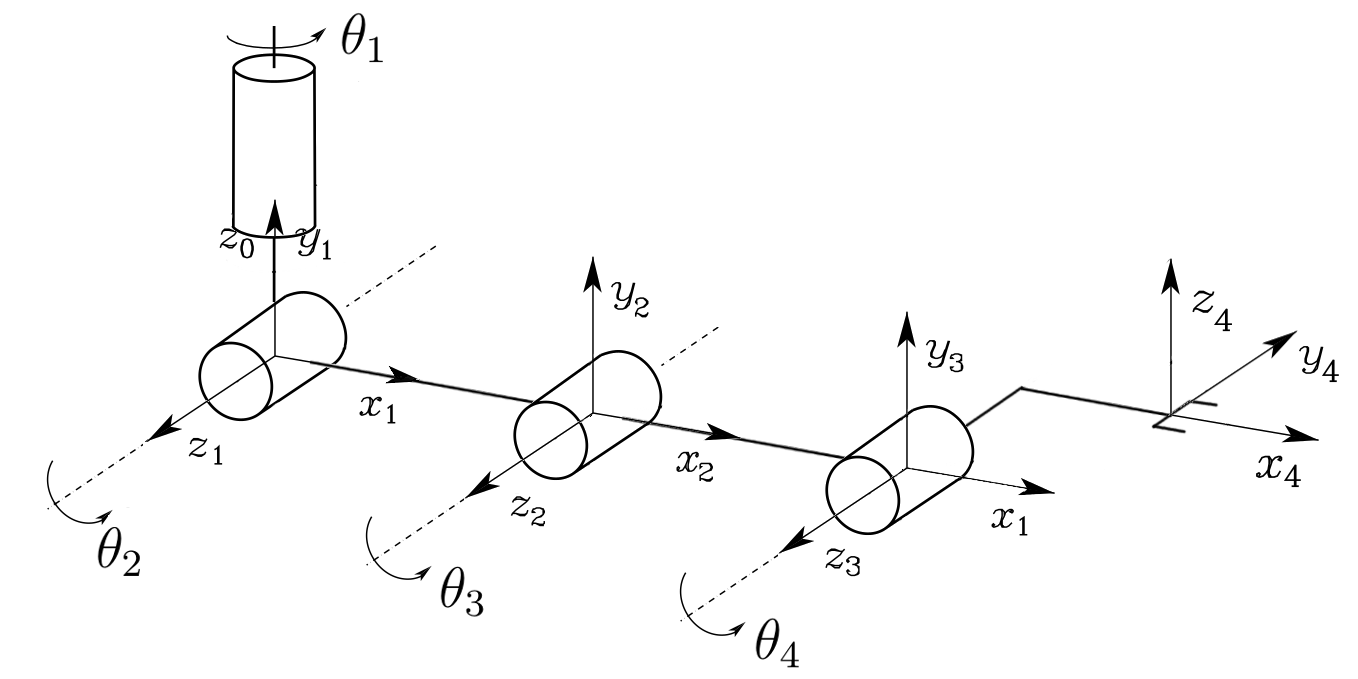
\includegraphics[width=0.9\linewidth]{./img/m2_meio_2.png}
  \caption{Modelagem do Manipulador Tetis e posicionamento dos sistemas de coordenadas}
  \label{fig:modelo_tetis}
\end{figure}%

\section{Cinemática Direta}
O primeiro passo ao modelar um manipulador robótico é encontrar a cinemática direta. Será utilizada a convenção de Denavit-Hartenberg para posicionar os sistemas de coordenadas e obter os parâmetros. Seguindo os passos descritos em \ref{sec:denavit} os sistemas de coordenadas foram posicionados da seguinte forma:

\begin{itemize}
\item Eixo $\vec{z}_0$ escolhido ao longo da Junta 1. Origem $O_0$ escolhida arbitrariamente de modo a coincidir com $O_1$ por simplicidade.  
\item Eixo $\vec{z}_1$ escolhido ao longo da Junta 2. Origem $O_1$ na intersecção entre $\vec{z}_0$ e $\vec{z}_1$. Eixo $\vec{x}_1$ na direção normal ao plano definido por $\vec{z}_0$ e $\vec{z}_1$ pois se interceptam. O sentido foi arbitrariamente escolhido na direção de avanço da cadeia por simplicidade.
\item Eixo $\vec{z}_2$ escolhido ao longo da Junta 3. Origem $O_2$ na junta 3 pois $\vec{z}_2$ e $\vec{z}_1$ são paralelas. Eixo $\vec{x}_2$ escolhido arbitrariamente ao longo de $\vec{x}_1$ pois a normal comum entre $\vec{z}_2$ e $\vec{z}_1$ não é unicamente definida.
\item Eixo $\vec{z}_3$ escolhido ao longo da Junta 4. Origem $O_3$ na junta 3 pois $\vec{z}_3$ e $\vec{z}_2$ são paralelas. Eixo $\vec{x}_3$ escolhido arbitrariamente ao longo de  $\vec{x}_2$ pois a normal comum entre $\vec{z}_3$ e $\vec{z}_2$ não é unicamente definida.
\item Como não existe junta 5, eixo $\vec{z}_4$ definido arbitrariamente. Origem $O_4$ na extremidade do efetuador final. Eixo $\vec{x}_4$ normal ao eixo $\vec{z}_3$.
\end{itemize}

A partir dos eixos posicionados conforme a figura \ref{fig:modelo_tetis} é possível obter os parâmetros na tabela \ref{tab:dh_tetis}. 


\begin{table}[h!]
\centering
\caption{Parâmetros Denavit–Hartenberg para manipulatodor Tetis}
\label{tab:dh_tetis}
\begin{tabular}{rrrrr} \hline
Elo & $a_i$ & $\alpha_i$ & $d_i$  & $\theta_i$ \\ \hline
1   & 0     & $\pi/2$    & 0      & $\theta_1$ \\
2   & $E_3$ & 0          & 0      & $\theta_2$ \\
3   & $E_4$ & 0          & 0      & $\theta_3$ \\
4   & $E_5$ & $-\pi/2$   & $-M_5$ & $\theta_4$ \\ \hline
\end{tabular}
\end{table}


\begin{itemize}
\item $a_1 = 0$  e $d_1 = 0$ pois $O_0$ e $O_1$ coincidem. $\alpha_1 = \pi/2$ ângulo entre $\vec{z}_0$ e $\vec{z}_1$ ao redor de $\vec{x}_1$.
\item $a_2 = E_3$ é a distância entre $\vec{z}_1$ e $\vec{z}_2$ ao longo de $\vec{x}_2$ que corresponde ao comprimento do elo 2. $\vec{z}_1$ e $\vec{z}_2$ são sempre paralelos logo $\alpha_2 = 0$. A distância $d_2$ entre $\vec{x}_1$ e $\vec{x}_2$ ao longo de $\vec{z}_1$ é zero. 

\item $a_3 = E_4$ é a distância entre $\vec{z}_2$ e $\vec{z}_3$ ao longo de $\vec{x}_3$ que corresponde ao comprimento do elo 3. $\vec{z}_2$ e $\vec{z}_3$ são sempre paralelos logo $\alpha_3 = 0$. A distância $d_3$ entre $\vec{x}_2$ e $\vec{x}_3$ ao longo de $z_2$ é zero. 

\item $a_4 = E_5$ é a distância entre $\vec{z}_3$ e $\vec{z}_4$ ao longo de $\vec{x}_4$. $\alpha_4 = -\pi/2$ é o ângulo entre $\vec{z}_3$ e $\vec{z}_4$ ao redor de $\vec{x}_4$, sendo portanto negativo. $d_4 = -M_5$ é a distância entre $\vec{x}_3$ e $\vec{x}_4$ ao longo de $\vec{z}_3$. 
\end{itemize}

Considerando a posição inicial da figura \ref{fig:modelo_tetis} todos os ângulos $\theta_i$ são dados diretamente pelas variáveis de junta, sem \textit{offsets}. 


Obtemos a partir da equação \eqref{eq:transform_dh} as transformações homogêneas entre sistemas de coordenadas consecutivos:
%\begin{align*}
%\bm{R}_{01} =
%\m{c_1 & 0 & s_1   \\
%   s_1 & 0 & -c_1  \\
%   0   & 1 &    0  \\} 
%& & \vec{\bm{p}}_{01} = 0
%\end{align*}
%\begin{align*}
%R_{12} = 
%\m{c_2 & -s_2 &  0  \\
%   s_2 &  c_2 &  0  \\
%   0   &    0 &  1  \\} 
%\end{align*}
%\begin{align*}
%R_{23} = 
%\m{c_3 & -s_3 &  0  \\
%   s_3 &  c_3 &  0  \\
%   0   &    0 &  1  \\} 
%\end{align*}
%\begin{align*}
%R_{34} = 
%\m{c_4 &  0 & -s_4  \\
%   s_4 &  0 &  c_4  \\
%   0   & -1 &    0  \\} 
%\end{align*}


%\begin{equation}
%\bm{R}_{04} = 
%\m{
%	c_1 c_{234} & -s_1 & -c_1 s_{234} \\
%	s_1 c_{234} & -c_1 & -s_1 s_{234} \\
%		s_{234} &    0 & 	  c_{234}
%}
%\end{equation}

\begin{align*}
{T}_{01} = 
\m{c_1 & 0 & s_1 &  0 \\
   s_1 & 0 & -c_1 & 0 \\
   0   & 1 &    0 & 0 \\
   0   & 0 &    0 & 1}
& &
{T}_{12} =  \m{c_2 & -s_2 &  0 & E_3 c_2 \\
   s_2 &  c_2 &  0 & E_3 s_2  \\
   0   &    0 &  1 & 	   0  \\
   0   &    0 &  0 &       1} 
\end{align*}

\begin{align*}
{T}_{23} = 
\m{c_3 & -s_3 &  0 & E_4 c_3 \\
   s_3 &  c_3 &  0 & E_4 s_3  \\
   0   &    0 &  1 & 	   0  \\
   0   &    0 &  0 &       1}
& &
{T}_{34} = 
\m{c_4 &    0 &  -s_4 & E_5 c_4 \\
   s_4 &    0 &   c_4 & E_5 s_4 \\
   0   &   -1 &     0 & 	-M_5 \\
   0   &    0 &     0 &       1}
\end{align*}


\begin{equation} \label{eq:cine_direta}
{T}_{04} = {T}_{01} {T}_{12}  {T}_{23} {T}_{34} = 
\m{
   c_1 c_{234} & -s_1 & -c_1 s_{234} & -M_5 s_1 + E_4 c_{23}c_1 + E_3 c_1 c_2 + E_5 c_{234} c_1 \\
   s_1 c_{234} & -c_1 & -s_1 s_{234} &   M_5 c_1+E_4 c_{23} s_1 + E_3 c_2 s_1 + E_5 c_{234} s_1 \\
   s_{234}     &    0 &      c_{234} &					     E_4 s_{23} + E_3 s_2 + E_5 s_{234} \\
   0   &    0 &     0 &      												   1
} 
\end{equation}

Definindo ${T}_{b0} = {I}$ e ${T}_{4e} = {I}$, pela equação \eqref{eq:base_efetuador} temos
\begin{equation}
{T}_{be} ({q}) = {T}_{04}({q})
\end{equation}


\section{Espaço das Juntas e Operacional}
Antes de tratar de estratégias de controle é necessário definir o espaço operacional e o espaço das juntas,  sob os quais serão aplicadas as leis de controle. 
Como trata-se de um manipulador 4-DOF de temos que o vetor do espaço operacional tem dimensão $(4 \times 1)$ dado por 
\begin{equation} \label{eq:operational_space}
{x_e} = \m{{p}_e \\ \phi_e}
\end{equation}
onde o vetor ${p}_e$ descreve a posição cartesiana representada no referencial da base:
\begin{equation}
{p}_e = \m{x \\ y \\ z}
\end{equation}
e $\phi_e$ é o grau de liberdade de orientação \textit{pitch}, dado por
\begin{equation} \label{eq:orientacao}
\phi_e = -(\theta_2 + \theta_3 + \theta_4)
\end{equation}

O espaço das juntas é definido por 
\begin{equation} \label{joint_space}
{q} = \m{q_1 \\ q_2 \\ q_3 \\ q_4} = \m{\theta_1 \\ \theta_2 \\ \theta_3 \\ \theta_4  }
\end{equation} 
pois todas as juntas são de revolução.

\section{Cinemática Diferencial}

\subsection{Jacobiano Analítico}
A partir da cinemática direta em \eqref{eq:cine_direta} e da equação \ref{eq:jacob_pos} podemos obter o Jacobiano de posição para o manipulador diferenciando a equação em relação as variáveis de junta. 
\begin{equation}
{p}_e = \m{x \\ y \\ z} =
\m{
   -M_5 s_1 + E_4 c_{23}c_1 + E_3 c_1 c_2 + E_5 c_{234} c_1 \\
     M_5 c_1+E_4 c_{23} s_1 + E_3 c_2 s_1 + E_5 c_{234} s_1 \\
   						 E_4 s_{23} + E_3 s_2 + E_5 s_{234} \\
}
\end{equation}

\begin{equation}
({J}_{ap})_b = 
\m{
	\ddfrac{\partial x}{\partial q_1} & \ddfrac{\partial x}{\partial q_2} & \ddfrac{\partial x}{\partial q_3} & \ddfrac{\partial x}{\partial q_4}  \\
	\ddfrac{\partial y}{\partial q_1} & \ddfrac{\partial y}{\partial q_2} & \ddfrac{\partial y}{\partial q_3} & \ddfrac{\partial x}{\partial q_4}  \\
	\ddfrac{\partial z}{\partial q_1} & \ddfrac{\partial z}{\partial q_2} & \ddfrac{\partial z}{\partial q_3} & \ddfrac{\partial z}{\partial q_4}  \\
}
\end{equation}
onde
\begin{align*}
&\frac{\partial x}{\partial q_1} =& - M_5c_1 - E_4c_{23}s_1 - E_3c_2s_1 - E_5c_{234}s_1  \\
&\frac{\partial x}{\partial q_2} =& -c_1(E_4s_{23}+E_3s_2+E_5s_{234}) \\
&\frac{\partial x}{\partial q_3} =& -c_1(E_4s_{23}+E_5s_{234}) \\
&\frac{\partial x}{\partial q_4} =& -E_5s_{234}c_1 \\
&\frac{\partial y}{\partial q_1} =& -M_5s_1+E_4c_{23}c_1+E_3c_1c_2+E_5c_{234}c_1 \\
&\frac{\partial y}{\partial q_2} =& -s_1(E_4s_{23}+E_3s_2+E_5s_{234}) \\
&\frac{\partial y}{\partial q_3} =& -s_1(E_4s_{23}+E_5s_{234}) \\
&\frac{\partial y}{\partial q_4} =& -E_5s_{234}s_1 \\ 
&\frac{\partial z}{\partial q_1} =& 0 \\ 
&\frac{\partial z}{\partial q_2} =& E_4c_{23}+E_3c_2+E_5c_{234} \\
&\frac{\partial z}{\partial q_3} =& E_4c_{23}+E_5c_{234}\\
&\frac{\partial z}{\partial q_4} =& E_{5}c_{234} 
\end{align*}

A partir de \ref{eq:jacob_or} e de \ref{eq:orientacao} podemos calular o Jacobiano de Orientação
\begin{equation}
{J}_{a\phi}({q}) = \frac{\partial \phi_e}{\partial {q}} = \m{0 & -1 & -1 & -1}
\end{equation}
 
Em alguns modos como controle por servo visão e no controle manual com joystick é interessante fazer o controle no referencial do efetuador, portanto precisamos representar o Jacobiano de posição no referencial do efetuador como $({J}_{ap})_e = {R}_{04}^T ({J}_{ap})_e$.  

\begin{equation}
({J}_{ap})_e =  
\m{
    -M_5c_{234} & E_3s_{34}+E_4s_4 & E_4s_4 & 0 \\
    E_4c_{23}+E_3c_2+E_5c_{234} & 0 & 0 & 0 \\
    M_5s_{23} &  E_5+E_3c_{34}+E_4c_4 & E_5+E_4c_4 & E_5 
}
\end{equation}


%A partir daqui, para simplificar a notação, sempre será referenciado o Jacobiano Analitico no referencial da base $(\bm{J}_A)_0$  como  $\bm{J}_0$ e o Jacobiano Analítico no referencial do efetuador $(\bm{J}_A)_N$ como $\bm{J}_N$.

%\section{Singularidades}

\section{Malha Aberta no Espaço Operacional} 
Este é um modo em malha aberta, onde o sinal de entrada no controlador é de velocidade no referencial da base ou do efetuador, ou seja a velocidade linear ${\dot{p}}_d$. Utiliza-se a equação \eqref{eq:jacob_pos} para calcular a velocidade de cada junta. 

\begin{figure}[h!]
\centering
\begin{tikzpicture}[auto, node distance=2cm,>=latex']
    % We start by placing the blocks
    \node [input, name=input] {};
    \node [block, right of=input] (J) {$J^{-1}$};
    \node [block, right of=J] (Integral) {$\int$};
    \node [output, right of=Integral] (output) {};

    \draw [draw,->] (input) -- node {$\dot{{x}}_e$} (J);
    \draw [->] (J) -- node {${\dot{q}}$} (Integral);
    \draw [->] (Integral) -- node [name=x] {${q}$}(output);
\end{tikzpicture}
\caption{Diagrama de Blocos: Modo de velocidade do Espaço Operacional}
\label{fig:vel_op}
\end{figure}


\subsection{Sistema de coordenadas da Base} \label{sec:openloopbase}
Quando o controle é feito no referencial da base ${\dot{x}}_d$ é velocidade desejada expressa no referencial da base e utiliza-se $({J}_{a})_e$.
\begin{equation}
{u} = {\dot{q}}_d = ({J}_{a})_b^{-1} ({\dot{x}}_d)_e
\end{equation}
\subsection{Sistema de coordenadas do Efetuador} \label{sec:openloopefct}
Quando o controle é feito no referencial do efetuador ${\dot{x}}_d$ é velocidade desejada expressa no referencial do efetuador e utiliza-se $({J}_{a})_e$.
\begin{equation}
{u} = {\dot{q}}_d = ({J}_{a})_e^{-1} ({\dot{x}}_d)_e
\end{equation}
onde 
\begin{equation}
{\dot{x}}_d = \m{{\dot{p}}_d \\ 0}
\end{equation}

\section{Controle de Posição no Espaço das Juntas} \label{sec:position_joint}
O controle de posição no espaço das juntas consiste em uma realimentação com controle proporcional individual para cada junta. Considerando que as juntas sejam modeladas como integradores, o diagrama \ref{fig:pos_juntas} mostra a malha de controle.

\begin{figure}[h!]
\centering
\begin{tikzpicture}[auto, node distance=2cm,>=latex']
    % We start by placing the blocks
    \node [input, name=input] {};
    \node [sum, right of=input] (sum) {};
    \node [block, right of=sum] (controller) {${K}_j$};
    \node [block, right of=controller] (system) {$\ddfrac{1}{s}$};
    % We draw an edge between the controller and system block to 
    % calculate the coordinate u. We need it to place the measurement block. 
    \draw [->] (controller) -- node[name=u] {${u}$} (system);
    \node [output, right of=system] (output) {};
    \node [tmp, below of=u] (tmp1) {};

    % Once the nodes are placed, connecting them is easy. 
    \draw [->] (system) -- node [name=s] {${q}$}(output);
    \draw [draw,->] (input) -- node {${q_d}$} (sum);
    \draw [->] (sum) -- node {${e}$} (controller);
    \draw [->] (s) |- (tmp1)-| node[pos=0.99] {$-$} node [near end] {${q}$} (sum);
       %\draw [->] (measurements) -| node[pos=0.99] {$-$} 
       % node [near end] {$\bm{q}_m$} (sum);
\end{tikzpicture}
\caption{Diagrama de Blocos: Modo de Posição no Espaço das Juntas}
\label{fig:pos_juntas}
\end{figure}

A lei de controle é dada por 
\begin{equation}
{u} = {K}_j ({q}_d - {q})
\end{equation}
onde ${K_j} = k_j {I}$.

\section{Controle de Posição no Espaço Operacional} \label{sec:pos_operacional}
Para este modo considera-se o problema de controle de posição no espaço operacional conforme definido em \ref{eq:op_space}. Para referências constantes, ou seja, quando $\dot{{x}}_d = 0$ a lei de controle dada por
\begin{equation} \label{eq:lei_posicao}
{u} = ({J}_{a})_b^{-1} {K}_p ({x_d} - {x_e})
\end{equation}
é capaz de levar o ${e} \rightarrow 0$ quando $t \rightarrow \infty$.

\section{Controle Proporcional com Feedforward} \label{sec:pplusf}
Para o rastreamento de trajetória considera-se o problema de seguir um referência no referencial da base ${x}_d(t)$ que é função do tempo, conhecidos ${x}_d(t)$ e ${\dot{x}}_d(t)$. Para levar o erro assintoticamente a zero, utiliza-se uma lei de controle proporcional com \textit{feedforward} utilizando a inversa do Jacobiano Analítico. Conforme mostrado em ~\ref{controle_cinematico}, a lei de controle dada por 
\begin{equation}
{u} = ({J}_{a})_b^{-1} (\dot{{x}}_d + {K}_t ({x_d} - {x_e}))
\end{equation} 
é capaz de levar o erro assintoticamente a zero pois a dinâmica fica 
\begin{equation}
\dot{{e}} + {K} {e} = 0
\end{equation}

O algoritmo de controle pode ser resumido por:
\begin{align}
{e} &= ({x}_d)_b- ({x_e})_b  \label{eq:error_pf}\\
{\bar{u}} &= {K}_t {e} + {\dot{x}}_d \\
{u} &= ({J}_a)_b^{-1} {\bar{u}}
\end{align}

%\begin{algorithm}
%\caption{<your caption for this algorithm>}
%\begin{algorithmic}
%\State $t = getTime()$
%\State $t = getTime()$
%\If {$i\geq maxval$}
%%    \State $i\gets 0$
%\Else
%    \If {$i+k\leq maxval$}
%        \State $i\gets i+k$
%    \EndIf
%\EndIf
%\end{algorithmic}
%\end{algorithm}

\section{Controle por Servo Visão} \label{sec:servo_vision}
O controle por servo visão no manipulador TETIS é feito através de uma configuração \textit{eye-in-hand}, onde a câmera é montada no efetuador final do manipulador, utilizando a abordagem de Servo Visão Baseada em Posição (PBVS). Na seção \ref{sec:minoru} é descrita a câmera utilizada. Trata-se de uma câmera estereoscópica, no entanto será utilizada apenas um dos sensores.

%\begin{figure}[H]
%\centering
%\begin{subfigure}{.5\textwidth}
%  \centering
%  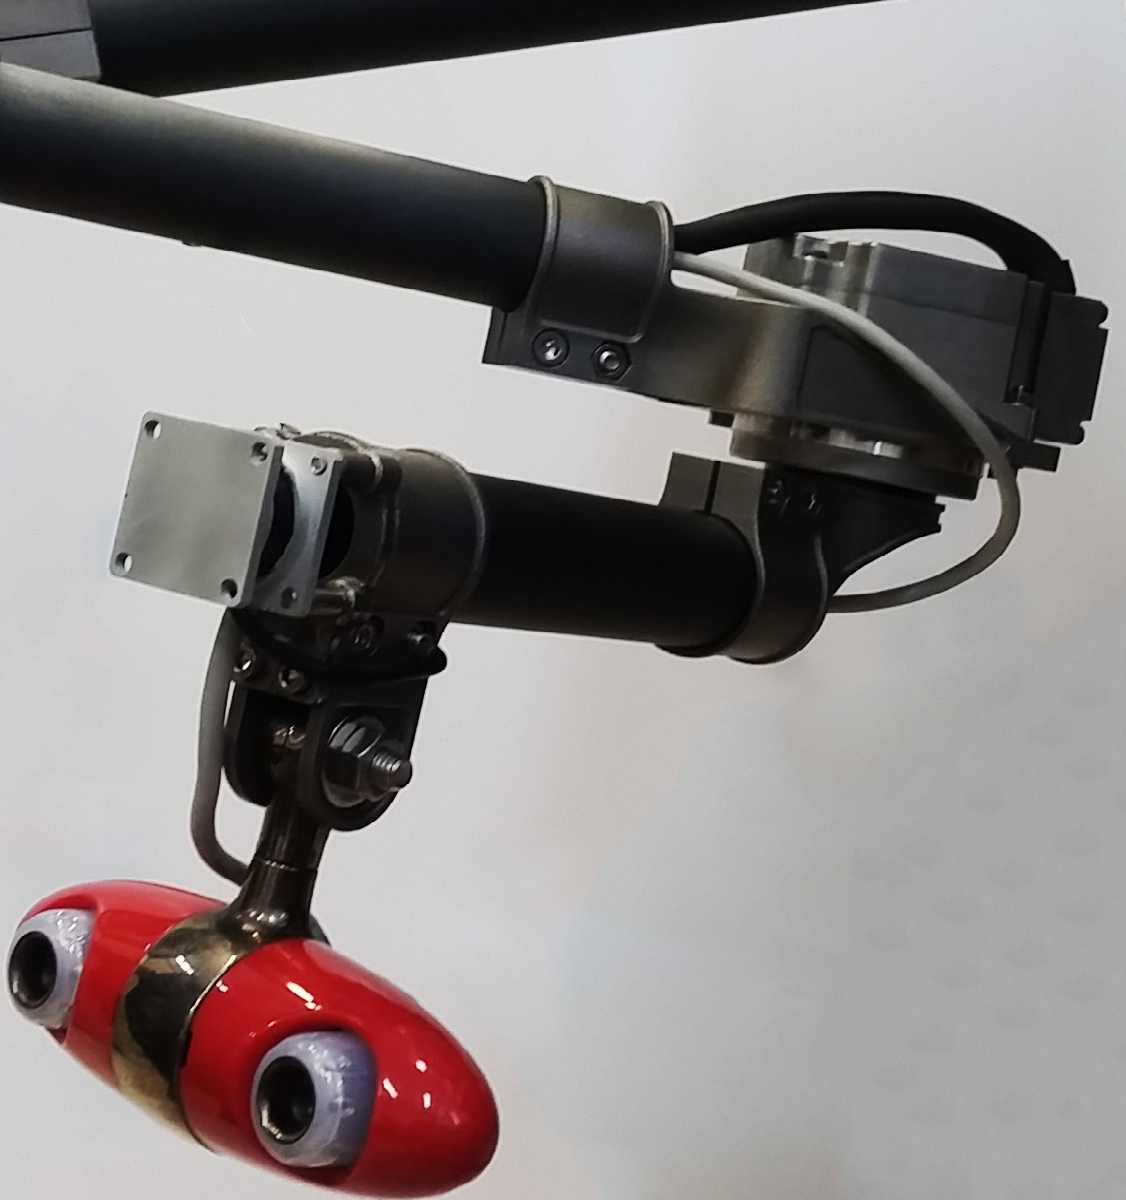
\includegraphics[width=\linewidth]{./img/manip_zoom.png}
%  \caption{Efetuador com câmera}
%  \label{fig:efetuador}
%\end{subfigure}%
%\begin{subfigure}{.5\textwidth}
%  \centering
%  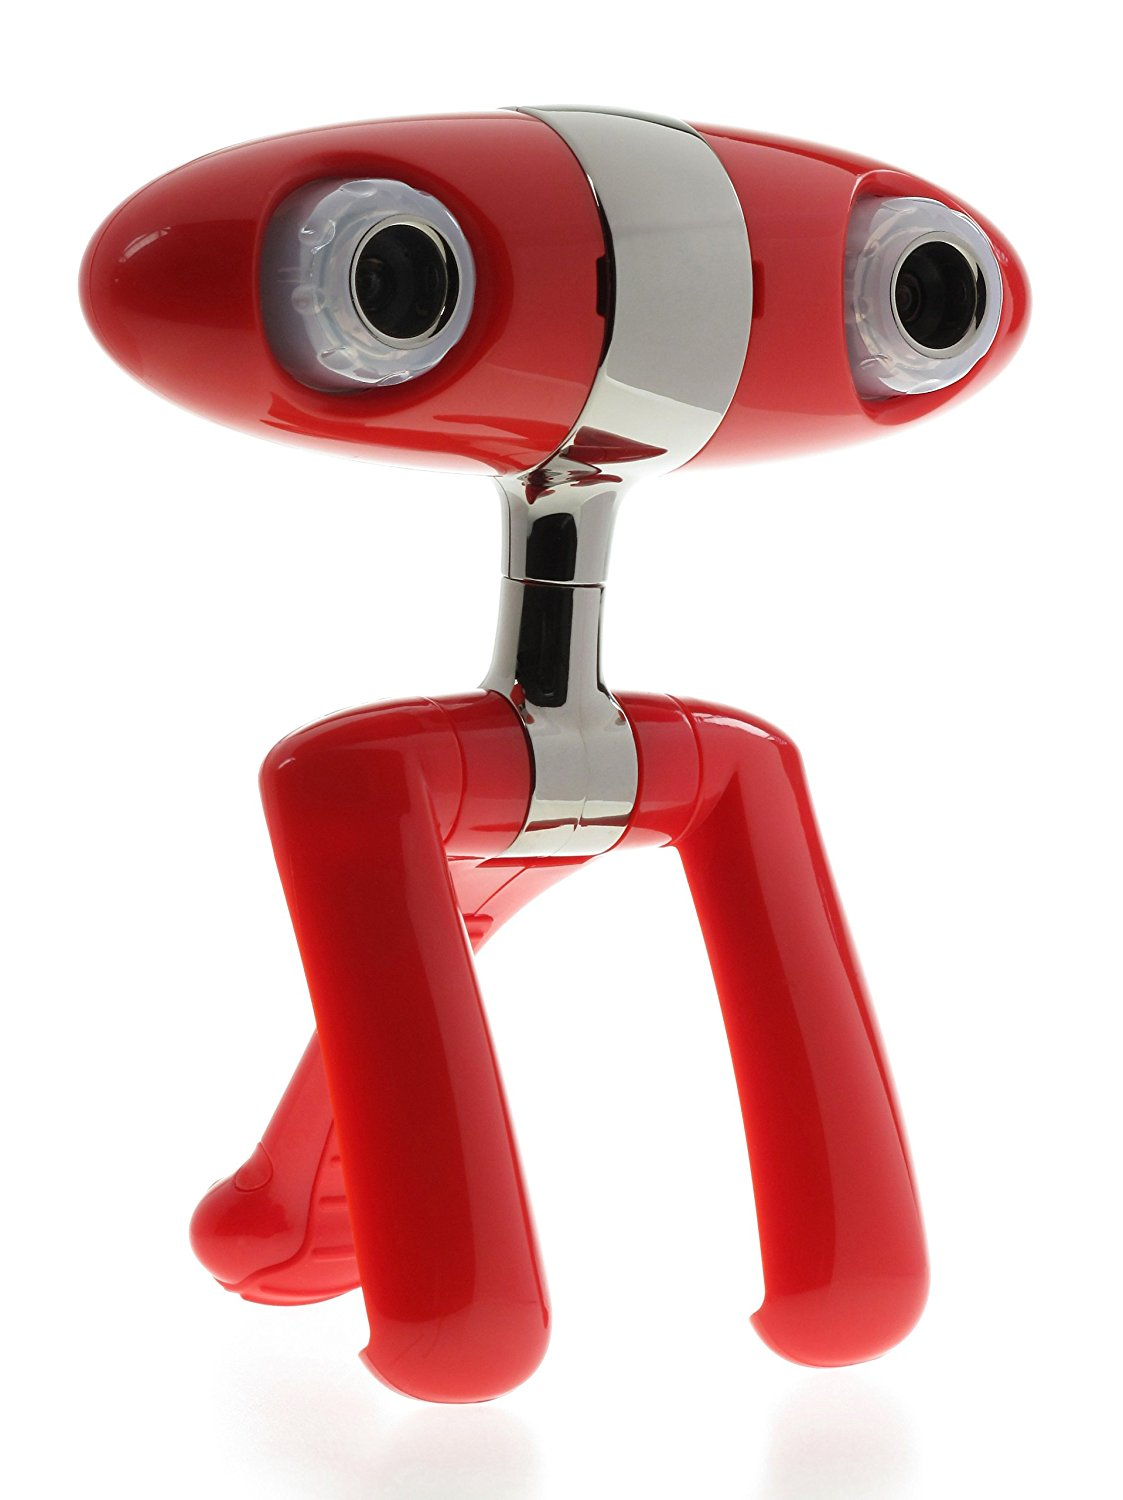
\includegraphics[width=0.8\linewidth]{./img/minoru.jpg}
%  \caption{Minoru Camera}
%  \label{fig:minoru}
%\end{subfigure}
%\label{fig:efet_minoru}
%\caption{Efetuador e câmera Minoru}
%\end{figure}


O objetivo é deste modo de controle é rastrear um alvo, que é representado por um QR code como o da figura \ref{fig:camera_target}. Deseja-se que o efetuador rastreie sempre a orientação normal ao plano do alvo.

A matriz de calibração ${K}$ da equação \eqref{eq:camera_projection} obtida através do processo descrito em \cite{calibration_tutorial} é:

\begin{equation}
{K} = \m {
	f/\rho_w & 0 & u_0 \\
	0        & f/\rho_h &v_0 \\
	0 & 0 & 1 \\
}
=
\m{
	877.62 	& 0 		& 306.53 \\
	0  		& 880.32 	& 210.12 \\
	0   	& 0 		& 1 \\	
}	
\end{equation}

Observando que o referencial da câmera e do efetuador são dados pela figura \ref{fig:camera_ref}, podemos chegar a seguinte transformação homogênea

\begin{equation} \label{eq:tec}
{T}_{ec} = \m{
	0 & 0 & 1 & -30 \\
	0 & -1 & 0 & 101 \\
	1 &  0 & 0 & -43 \\
	0 &  0 & 0 &  1
}
\end{equation}

\begin{figure}[!h]
  \centering
  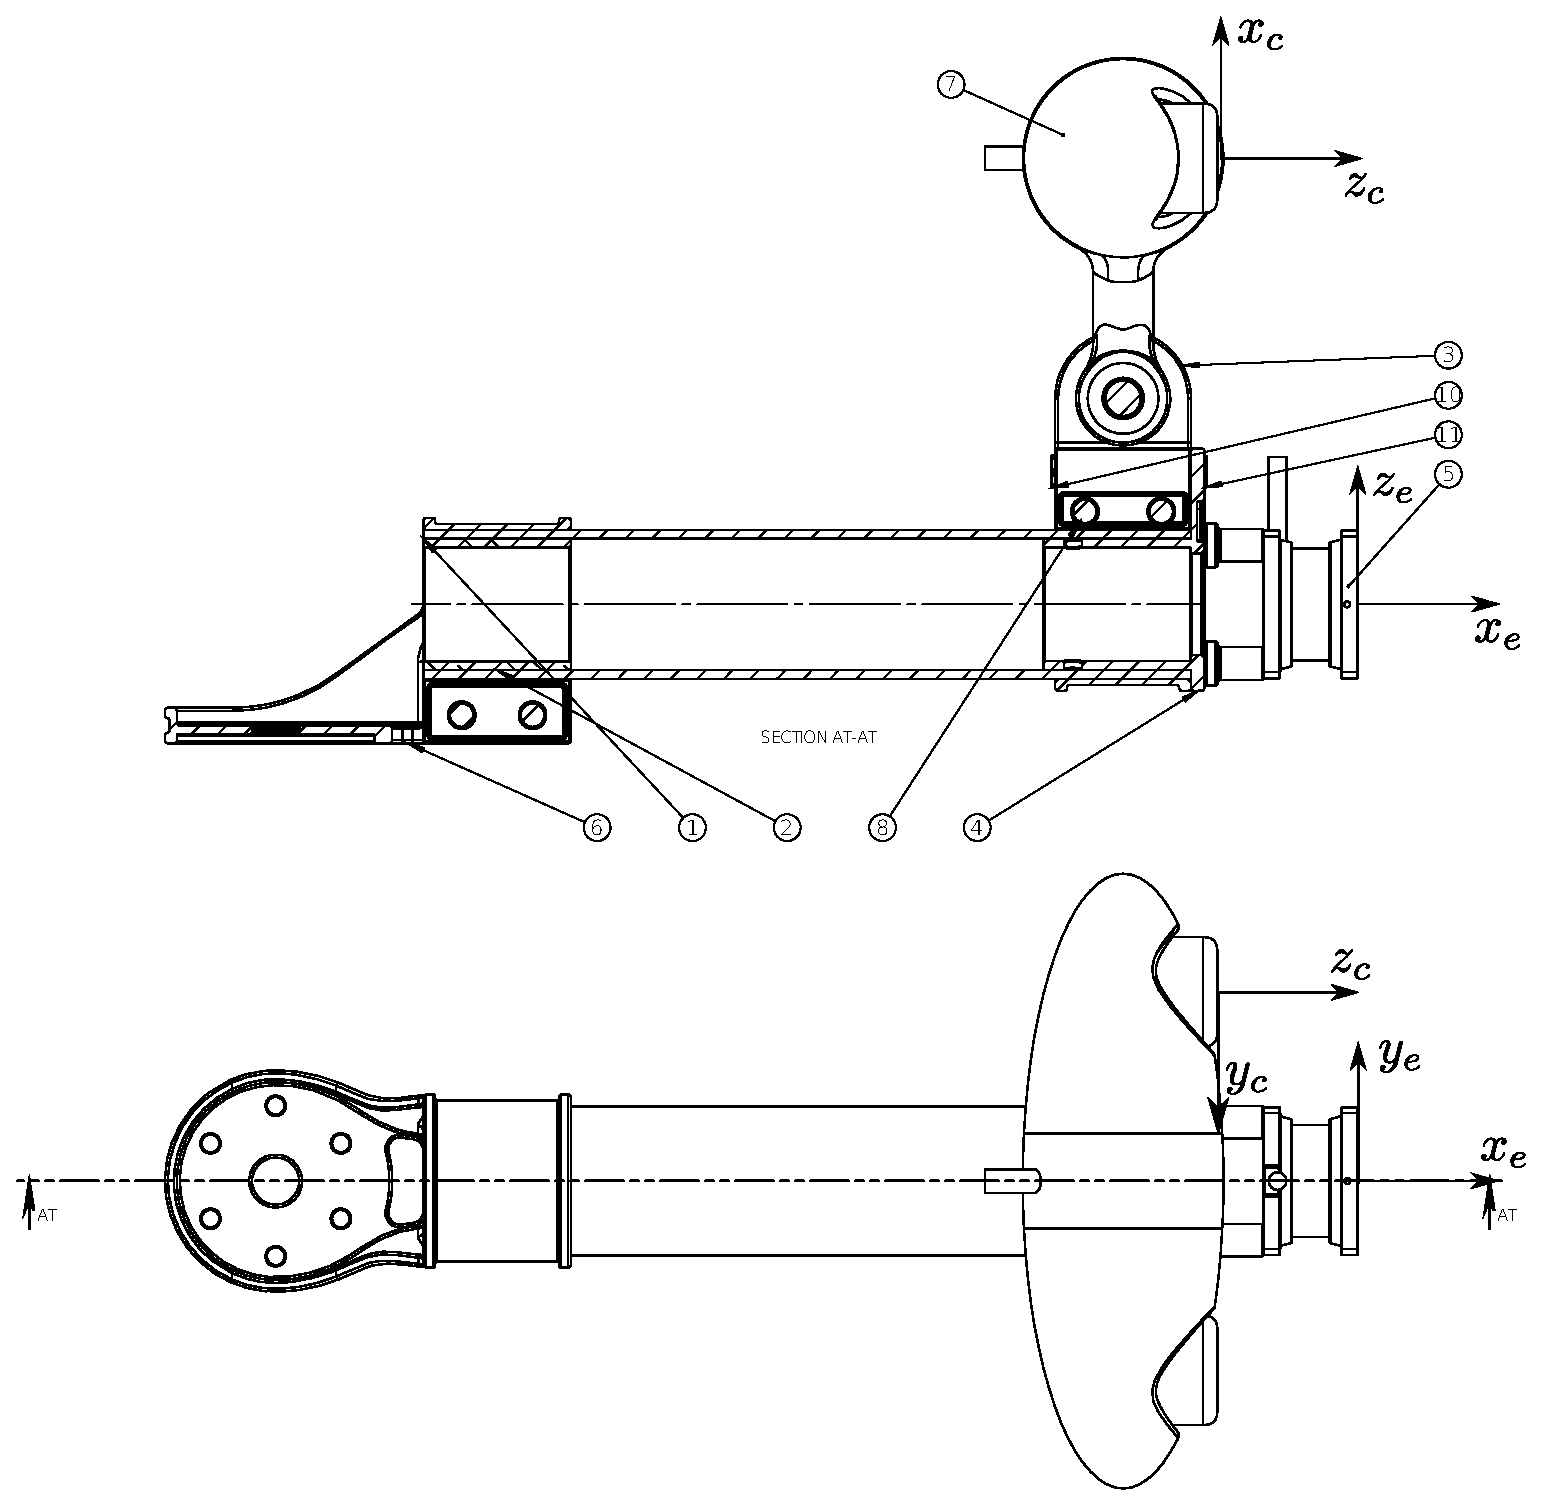
\includegraphics[width=0.8\linewidth]{./img/effector2}
  \caption{Sistemas de coordenadas da câmera e do efetuador}
  \label{fig:camera_ref}
\end{figure}

\begin{figure}[!h]
  \centering
  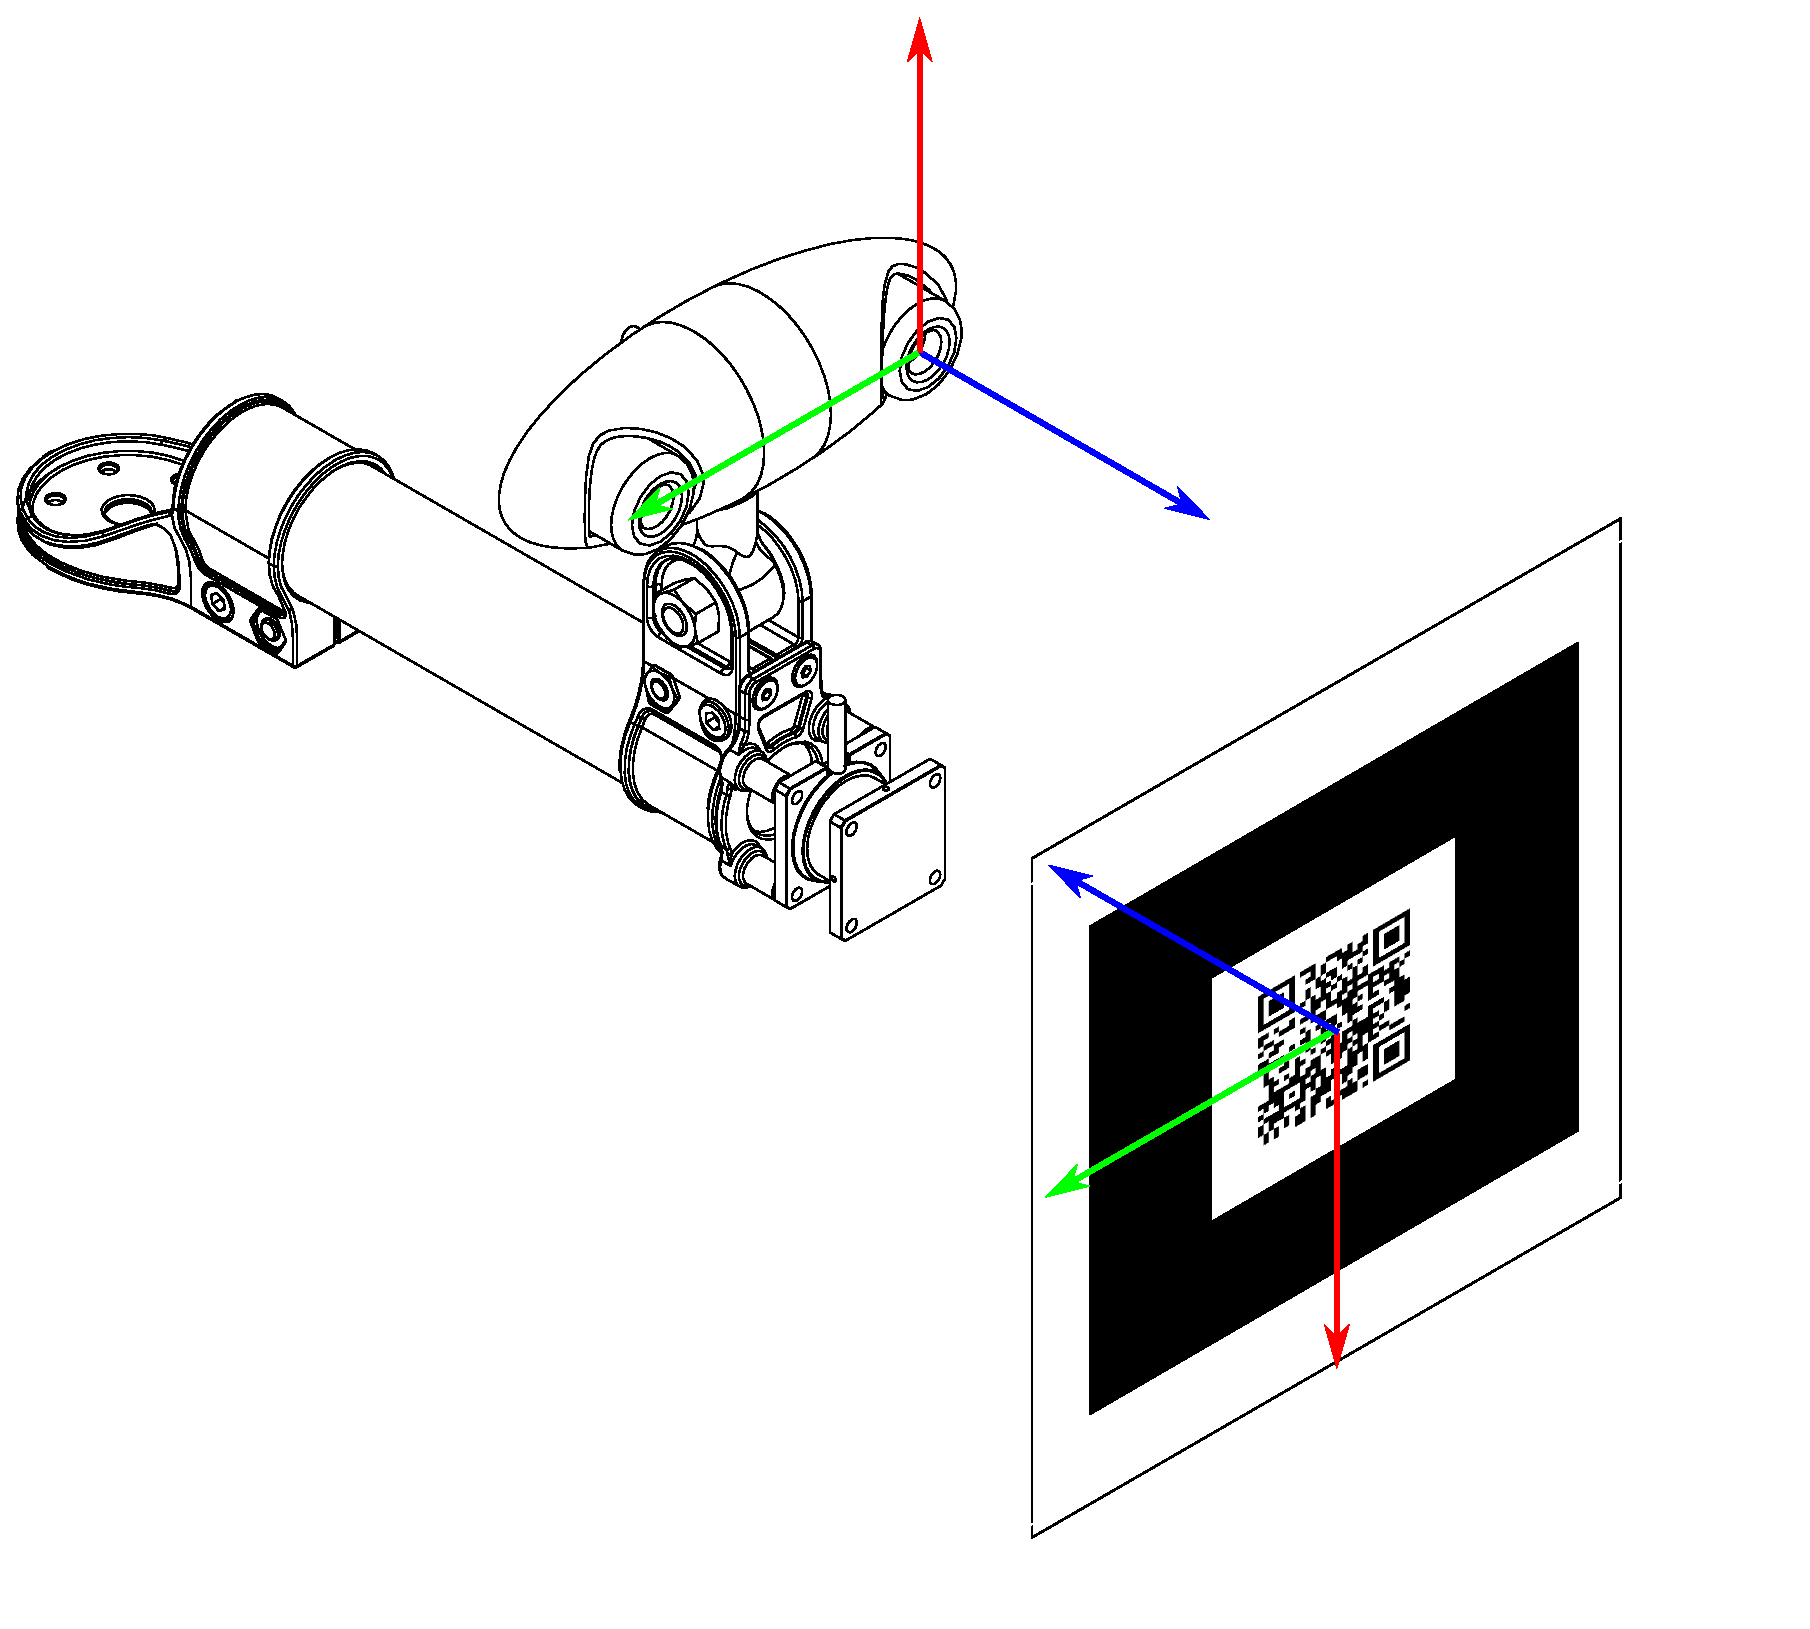
\includegraphics[width=0.8\linewidth]{./img/camera_target}
  \caption{Sistemas de coordenadas da câmera e do alvo}
  \label{fig:camera_target}
\end{figure}


Para a servo visão baseada em posição, foi utilizada uma lei de controle proporcional
\begin{equation} \label{eq:lei_posicao}
{u} = ({J}_{a})_e^{-1} {K}_t [({x}_t)_e - ({x_e})_e]
\end{equation}
onde ${x}_t$ e ${x_e}$ estão representados no referencial do efetuador. Portanto precisamos saber a posição e orientação ${x}_t$ do alvo em relação ao efetuador
\begin{equation}
{T}_{et} = {T}_{ec} {T}_{ct}
\end{equation}
onde ${T}_{ec}$ é dado por \eqref{eq:tec} e ${T}_{ct}$ obtemos através de algoritmos de estimação de posição e orientação a partir de visão computacional. 

\begin{equation}
({x}_t)_e = \m{ ({p}_t)_e \\ \phi_t }
\end{equation}
onde $({p}_t)_e$ é o vetor de translação que pode ser obtido diretamente de ${T}_{ec}$ e  $\phi_t$ é a orientação, que pode ser obtido de duas formas.


%TODO
A primeira alternativa é obter a rotação em torno do eixo $x$ (\textit{pitch}) em relação ao referencial do efetuador, extraído de ${T}_{et}$. No entanto essa opção não permite que o alvo seja rotacionado em torno de ${z}_c$, pois a rotação em torno de ${x}_c$ não mais representará a inclinação do plano do alvo em relação a posição inicial, que faz o efetuador rastrear a direção normal ao alvo. A figura \ref{fig:projection} ilustra isso. 

Portanto, optou-se pela segunda alternativa. Projeta-se o eixo do alvo $({z}_t)_c$, representado do referencial da câmera, no plano $({z}_{t_0})_c \times ({x}_{t_0})_c$, onde $({z}_{t0})_c$ indica o eixo de coordenadas do alvo $z_t$ em sua posição inicial conforme a figura \ref{fig:camera_target}. Em seguida encontra-se o ângulo entre os vetores $({z}_{t_0})_c$ e $({z}_{t_0})_c$. 

\begin{figure}[!ht]
\centering
  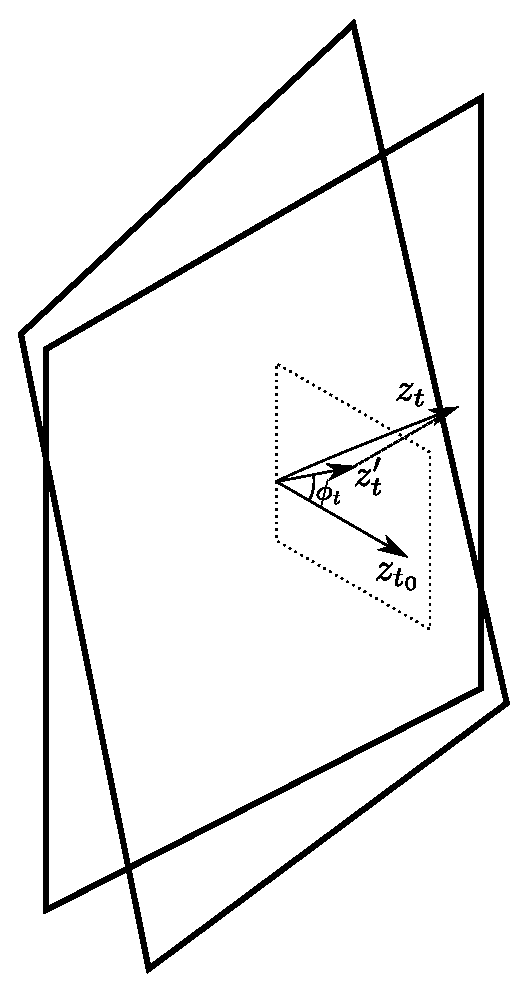
\includegraphics[width=0.3\linewidth]{./img/projection.eps}
  \caption{Caso em que a rotação em torno de ${x}_c$ não representa a inclinação do plano do alvo.}
  \label{fig:projection}
\end{figure}%


Dada a matriz de rotação ${R}_{ct_0}$, da câmera à posição inicial
\begin{equation}
{R}_{ct_0} = \m{ ({x}_{t_0})_c & ({y}_{t_0})_c  & ({z}_{t_0})_c} = 
\m{
	0 & 1 & 0 \\
	1 & 0 & 0 \\
	0 & 0 & -1
}
\end{equation}
é conhecida a normal ao plano do alvo é ${n} = {x}_{t_0} \times {z}_{t_0} =  {y}_{t_0} $. A matriz de projeção linear \citep{strang} de um vetor em um plano é dada por
\begin{equation}
{P} = {I} - {n} {n}^T,
\end{equation}
logo para ${n} = {y}_{t_0}$ temos 
\begin{equation}
{P} =  \m{
	 0  &   0  &   0 \\
     0  &   1  &   0 \\
     0  &   0  &   1
}.
\end{equation}

O vetor projetado no plano é dado por
\begin{equation}
{z'}_{t} = {P} {z}_{t},
\end{equation}
assim basta apenas encontrar o ângulo entre os vetores ${z'}_{t}$ e ${z}_{t_0}$, que pode ser calculado pela fórmula do Cosseno \citep{strang} 
\begin{equation}
\phi_t = \cos^{-1} \left( \frac{{z'}^T_{t} {z}_{t_0} } {||{z'}_{t}|| \; ||{z}_{t_0}||} \right)
\end{equation}


%\begin{align}
%(\bm{p}_t)_e &= (\bm{p}_c)_e + (\bm{p}_t)_e \\
%(\bm{p}_t)_e &= (\bm{p}_c)_e + \bm{R}_{ec} (\bm{p}_t)_c 
%\end{align}


Após obter os valores de $(p_t)_e$ e $\phi_t$, sabemos $(x_t)_e$ e controle se resume a:
\begin{align}
{e} &= ({x}_t)_e - ({x})_e \\
{\bar{u}} &= {K}_v {e}  \\
{u} &= ({J}_{a})_e^{-1} {e}
\end{align}

\section{Controle de Força} \label{sec:force}

Utilizando o sensor de força descrito em \ref{sec:optoforce}, montado no efetuador final do manipulador, deseja-se fazer o controle da força aplicada sobre uma superfície. 

A matriz de rotação do referencial do sensor para o referencial do efetuador, como definido em \ref{fig:modelo_tetis} é dada por

\begin{equation}
R_{es} = \m{
  0 & 0 & 1 \\
  0 & -1 & 0 \\
  1 & 0 & 0
}
\end{equation}

\subsection{Float}  \label{sec:forca_float}
Esse mode de controle de força consiste em configurar uma referência de controle de força ${f}_d = 0$, de modo que o efetuador do manipulador fique "flutuando", se movendo de forma sensível ao toque.

Primeiramente a força representada no referencial do sensor $({f})_s \in \mathbb{R}^3 $ é representada na base por $({f})_e = R_{es} ({f})_s$.
Como ${f}_d = 0$:
\begin{equation}
({e}_f)_e = - ({f})_e \\
\end{equation}

Utilizando um controle proporcional:
\begin{align}
\bar{{u}}_f &= {K}_f ({e}_f)_e \\
\bar{{u}} &= \m{ \bar{{u}}_f & 0}^T\\
{u} &= ({J_a})_b^{-1} \bar{{u}}
\end{align}

\subsection{Approach} \label{sec:forca_approach}
Considera-se o problema de controle de força na direção de \textit{approach} para o manipulador robótico 4-DOF em questão. O objetivo de controle é resolver o problema de \textit{set-point}, ou seja, rastrear uma referência de força constante.

É possível modelar o ambiente (força de contato), ou seja, a placa de poliestireno, como uma mola linear, através da \textit{Lei de Hooke}: 
\begin{equation}
f = -k_s (x - x_s)
\end{equation}
onde $x$ é a posição do ponto de contato com a superfície e $x_s$ um ponto na superfície.

Considerando que o controle de força seja ativado somente após a etapa de contato com o ambiente onde será aplicada a força e que o controle de força é feito apenas na direção de approach (segundo o sistema de coordenadas $\bar{E}_e$, na direção $x$), pode-se utilizar a malha de controle mostrada na figura \ref{fig:controle_forca}.

É utilizada uma lei de controle com ação proporcional e integral:
\begin{equation}
\bar{u} = -K_s^{-1} (K_fe_f + K_i \int_0^t e_f(\tau)d\tau)
\end{equation}


\begin{figure}[h!]
\centering
\begin{tikzpicture}[auto, node distance=2cm,>=latex']
    % We start by placing the blocks
    \node [input, name=input] {};
    \node [sum, right of=input] (sum) {};
    \node [block, right of=sum] (Ks1) {$k_s^{-1}$};
    \node [block, right of=Ks1] (C) {$C(s)$};
    \node [blockbig=right:C] (J) [right=1cm of C] {$(J_a)_e^{-1}$};
    \node [block=right:J] (Integral) [right=1cm of J] {$\int$};
    \node [blockbig, right of=Integral] (DirKine) {${k}(\cdot)$};

	\node [tmp=below:J] (tmp0) [below left=-1.25cm and .7cm of J] {};
	\node [tmp=below:J] (tmp00) [below left=-2cm and 0.7cm of J] {};
	\node [tmp=below:J] (tmp000) [below left=-2cm and 0cm of J] {};

    \node [tmp=below:J] (tmp1) [below left=-1.5cm and 0.5cm of J] {};
    \node [tmp=below:J] (tmp2) [below left=-1.5cm and 0cm of J] {};

    \node [tmp=below:J] (tmp3) [below left=-1cm and 0.5cm of J] {};
    \node [tmp=below:J] (tmp4) [below left=-1cm and 0cm of J] {};

    \node [tmp=below:J] (tmp5) [below left=-0.5cm and 0.5cm of J] {};
    \node [tmp=below:J] (tmp6) [below left=-0.5cm and 0cm of J] {};

    \node [tmp=below:J] (tmpk0) [below right=-2cm and 0cm of DirKine] {};
	\node [tmp=below:J] (tmpk00) [below right=-2cm and 0.7cm of DirKine] {};
	\node [tmp=below:J] (tmpk000) [below right=-1.25cm and 0.7cm of DirKine] {};

    \node [tmp=below:J] (tmpk1) [below right=-1.5cm and 0.5cm of DirKine] {};
    \node [tmp=below:J] (tmpk2) [below right=-1.5cm and 0cm of DirKine] {};

    \node [tmp=below:J] (tmpk3) [below right=-1cm and 0.5cm of DirKine] {};
    \node [tmp=below:J] (tmpk4) [below right=-1cm and 0cm of DirKine] {};

    \node [tmp=below:J] (tmpk5) [below right=-0.5cm and 0.5cm of DirKine] {};
    \node [tmp=below:J] (tmpk6) [below right=-0.5cm and 0cm of DirKine] {};


    \node [block=right:DirKine] (ks) [right=1cm of DirKine] {$k_s$};
    \node [output, right of=ks] (output) {};

    % Once the nodes are placed, connecting them is easy. 
    \draw [draw,->] (input) -- node {$f_d$} (sum);
    \draw [->] (sum) -- node {$e_f$} (Ks1);
    \draw [->] (Ks1) -- node {} (C);
    %\draw [->] (C) -- node[name=u] {$u$} (tmp0);
    \draw [->] (J) -- node {${\dot{q}}$} (Integral);
    \draw [->] (Integral) -- node {${q}$} (DirKine);
    \node [block, below of=J] (measurements) {$H(s)$};
    %draw [->] (DirKine) -- node {} (ks);
    \draw [->] (ks) -- node [name=x] {$f$}(output);
    \draw [->] (x) |- (measurements);
    \draw [->] (measurements) -| node[pos=0.99] {$-$} 
        node[near end] {$f_m$} (sum);

    \draw [->] (C) -- (tmp0) -|  (tmp00) |- node[pos=0.65] {$x$} (tmp000);

    \draw [->] (tmpk0) -- node[pos=0.2] {$x$} (tmpk00) -|  (tmpk000) |-  (ks);
    \draw [->] (tmp1) -- node[pos=0] {$y$} (tmp2);
    \draw [->] (tmp3) -- node[pos=0] {$z$} (tmp4);
    \draw [->] (tmp5) -- node[pos=0] {$\phi$} (tmp6);

    \draw [->] (tmpk2) -- node[pos=0.3] {$y$} (tmpk1);
    \draw [->] (tmpk4) -- node[pos=0.3] {$z$} (tmpk3);
    \draw [->] (tmpk6) -- node[pos=0.3] {$\phi$} (tmpk5);
    %\draw [->] (x) |- (tmp1) -| node[pos=0.9] {$-$} (sum);
\end{tikzpicture}
\caption{Diagrama de Blocos: Malha de Controle de Força.}
\label{fig:controle_forca}
\end{figure}

O diagrama \ref{fig:controle_forca} pode ser simplificado se abstrairmos as outras dimensões que não a de approach, resultando em \ref{fig:controle_forca_simples}.

\begin{figure}[h!]
\centering
\begin{tikzpicture}[auto, node distance=2cm,>=latex']
    % We start by placing the blocks
    \node [input, name=input] {};
    \node [sum, right of=input] (sum) {};
    \node [block, right of=sum] (Ks1) {$k_s^{-1}$};
    \node [block, right of=Ks1] (C) {$C(s)$};
    \node [block, right of=C] (PWM) {$k_s$};
    \node [block, right of=PWM] (Robo) {$\ddfrac{1}{s}$};
    \node [tmp, below of=K] (tmp1){};
    \node [output, right of=Robo] (output) {};

    % Once the nodes are placed, connecting them is easy. 
    \draw [draw,->] (input) -- node {$f_d$} (sum);
    \draw [->] (sum) -- node {$e_f$} (Ks1);
    \draw [->] (Ks1) -- node {} (C);
    \draw [->] (C) -- node[name=u] {$u$} (PWM);
    \node [block, below of=u] (measurements) {$H(s)$};
    \draw [->] (PWM) -- node [name=tau] {} (Robo);
    \draw [->] (Robo) -- node [name=x] {$f$}(output);
    \draw [->] (x) |- (measurements);
    \draw [->] (measurements) -| node[pos=0.99] {$-$} 
        node[near end] {$f_m$} (sum);
    %\draw [->] (x) |- (tmp1) -| node[pos=0.9] {$-$} (sum);
\end{tikzpicture}
\caption{Diagrama de Blocos: Malha de Controle de Força Simplificada.}
\label{fig:controle_forca_simples}
\end{figure}

Considerando $H(s) = 1$
\begin{equation}
G(s) = \frac{k_p s + k_i}{s^2 + k_p s + k_i}
\end{equation}

Como o sinal vindo do sensor é bastante ruidoso, utiliza-se um filtro de primeira ordem com $f_c = 1$.
\begin{equation}
H(s) = \frac{1}{\tau s + 1}
\end{equation}
onde $\tau = 1/(2 \pi f_c) = 0.159154943$.

Ficamos com a função de transferência a seguir a partir da qual é possível sintonizar os parâmetros do controlador.
\begin{equation}
G(s) = \frac{k_p \tau s^2 + (k_p + \tau k_i)s + k_i}{\tau s^3 + s^2 + k_p s + k_i}
\end{equation}

Considerando que obtemos do sensor de força um vetor $({f})_s \in \mathcal{R}^3$, representado no referencial do sensor. O controle de força pode ser implementado a partir das seguintes equações:
\begin{align}
({f})_e &= {R}_{es} ({f})_s \\
({e}_f)_e &= {f}_d - ({f})_e \\
\end{align}

A estratégia de controle PI é dada por
\begin{equation}
\bar{{u}}_f = -{K}_s^{-1} ({K}_f ({e}_f)_e + {K}_i \int_0^t ({e}_f)_e (\tau)d\tau)\\
\end{equation}

Como ${u} \in \mathcal{R}^4$  e desejamos controlar somente a direção de \textit{approach}:
\begin{equation}
\bar{{u}} = \m{ {S}_f \bar{{u}}_f \\ 0} 
\end{equation}
onde 
\begin{equation}
{S}_f = \m{
  1 & 0 & 0 \\
  0 & 0 & 0 \\
  0 & 0 & 0
},
\end{equation}
portanto:
\begin{equation}
{u} = ({J_a})_e^{-1} \bar{{u}}
\end{equation}

%Especificações:
%\section{Controle Híbrido}
%Considerando o diagrama \ref{fig:controle_forca}, é possível suprir os graus de liberdade não controlados $y$, $z$ e $\phi$ %com outra lei de controle, como por exemplo o um Proporcional com Feedforward de modo a aplicar uma força na direção de %approach e traçar uma trajetória de na superfície em que a força está sendo aplicada. 

%\section{Master-Slave (Omni)}
%TODO

% TODO: TABELA COM LEIS DE CONTROLE E FONTE DOS DADOS 